\documentclass{article}

\usepackage{graphicx}
\usepackage[margin=1 in]{geometry}

\DeclareGraphicsExtensions{.png,.jpg}

\begin{document}

\begin{center}

    \huge{\textbf{WhiteBoard}}

    \huge{\textit{An Efficient and Intuitive Learning Management System}}

    \huge{Project Progress Report}

    \vspace{10 pt}

    \large{
        \begin{tabular}{cccc}
            Noah Christiano&Joel Kottas&Shir Maimon&Jacob Roschen\\
        \end{tabular}
    }

\end{center}

\vspace{10 pt}

\section{Background}

A Learning Management System(LMS) is an interface between students, professors,
and school administration. One of the most popular LMSes, especially at
colleges and universities, is Blackboard\cite{Blackboard}. Blackboard, however,
is extremely slow and has unnecessary features that are often left unused. For
example, Blackboard's personalize page features are rarely used, and students
avoid the discussion boards. These LMSes' designs often make them difficult to
navigate. For example, Blackboard has two sets of navigation tabs, and it is
not obvious what the difference between them is. These problems add up to
create an interface that is slow and difficult to use, even though there is no
need for it to be that way. Students today would rather get what they need
quickly than have hundreds of features that they rarely, if ever, use. Other
LMSes include Moodle\cite{Moodle}, Veracross\cite{Veracross}, and
Canvas\cite{Canvas}. Moodle is open-source, but it is difficult to use.
Veracross is nice, but expensive. Canvas is more like Blackboard and is just
not good.

\section{Objective}

WhiteBoard will focus on having an efficient, intuitive interface, and it will
have features of excellent quality rather than a large quantity of features. It
is open-source, allowing it to be customized and used as desired, although it
focuses on the University of Rochester. Also, WhiteBoard will have a unified
user experience. It shouldn't take a student who is majoring in computer
science three days to find where the grades are posted, and even then to be
confused about what their grade is, and it should be easy to navigate to the
University of Rochester website. WhiteBoard's design will make such navigation
a pleasure.

\section{Features}

Specifically, WhiteBoard will have the following features:
\begin{itemize}
    \item Lightning-quick load times
    \item A secure and painless login system
    \item Course system, with registration and grades for students
    \item Convenient communication between administrators, professors, and
        students, both for general communication and announcements
    \item Open source
\end{itemize}

\section{Current Assets}

Our team's combined experience covers PHP and Javascript very well, the LAMP
stack and all its associated programming languages, and even configuring a
Linux server for web hosting. Everyone on the team understands design, and how
to learn from both the successes and the mistakes of systems like Blackboard.
As students, we have constant access to Blackboard, and we have the expertise
to dive into the site to see what code works well and what code doesn't. We are
also constantly learning, and our ability in areas relating to this project
will only increase.

We are also using several libraries to assist in creating WhiteBoard. We are
using jQuery, a javascript library, and code from the open source PHP-Login
project, so that we have a secure but simple to use system. The PHP-Login
library also includes a module for sending email, so we don't need to deal with
the intricacies of that. There are also many other libraries for Javascript and
PHP available should we find them useful.

The server we are using is an Apache server on Ubuntu. We're using an Amazon
EC2 free tier for testing and debugging. This won't work for any kind of
production use, but it's fine for testing and debugging.

We're also using PHPMyAdmin and MySQL Workbench for designing and managing the
database.

\section{Budget}

Because we aren't spending any money on a server for development, there are for
the most part no costs. However, if this site were to go into production, then
we would need a dedicated server, which would cost money.

\section{Development Environment}

We are collaborating over GitHub, which combines version control, file sharing,
and the ability to edit files online into one service.

Some people have a local server for testing code directly on their computers.
Others are unable to set this up, but this is not a problem since we have our
testing and debugging server that we can use.

\section{WhiteBoard, Currently}

We have made significant progress on WhiteBoard. We've designed and set up the
database, general layout of the website, and login system, and courses are
almost completely implemented.

\subsection{Database Structure}

We have thoroughly planned the database for the entire system. The database is
a MySQL relational database. Rather than trying to store too much data, and in
an effort to make the database as efficient as possible, we are using only 14
tables, as we show in figure \ref{fig:db}. This is far less than the
approximately 200 tables that Moodle uses.

\begin{figure}
    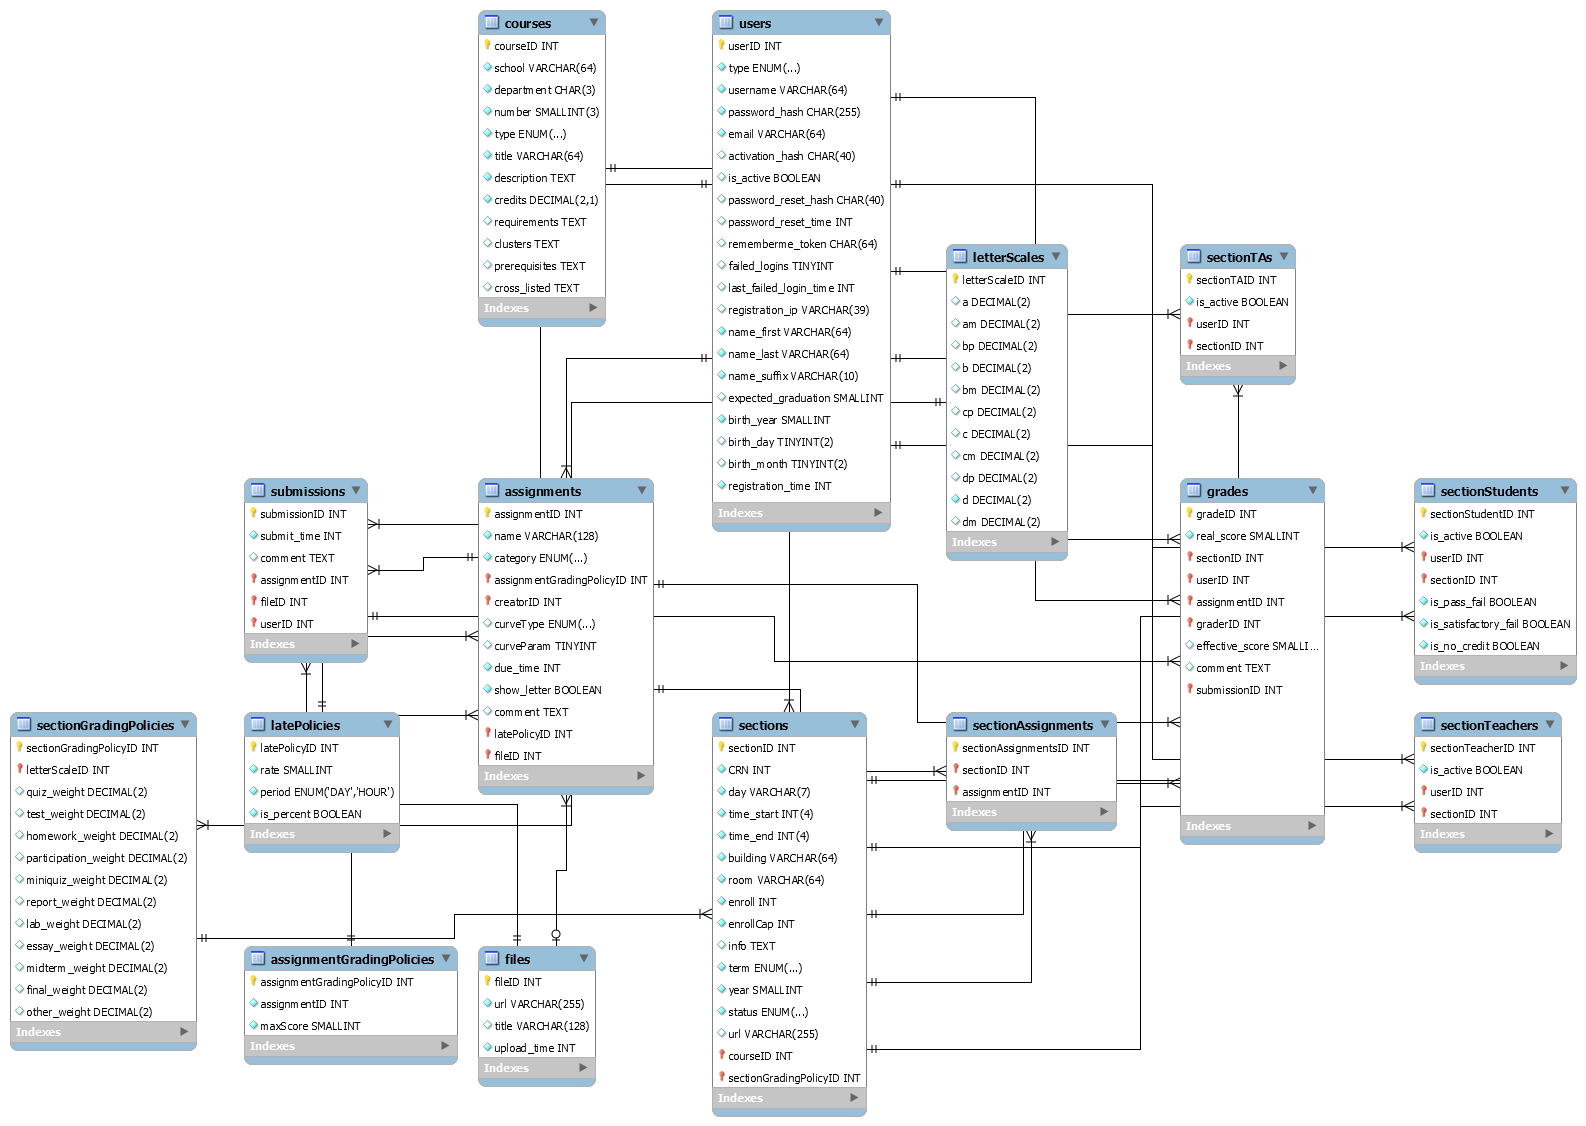
\includegraphics[width=\linewidth]{db}
    \caption{The database diagram, generated by MySQL Workbench.}
    \label{fig:db}
\end{figure}

\subsection{General Layout}

The general layout of the page is straightforward: there is a header with a
search bar and user info, a sidebar with tabs, and the main content area, as we
show in figure \ref{fig:gl}. The goal of this project is not to make anything
too fancy, and keeping the user interface simple like this is one of the main
ways we accomplish this goal.

\begin{figure}
    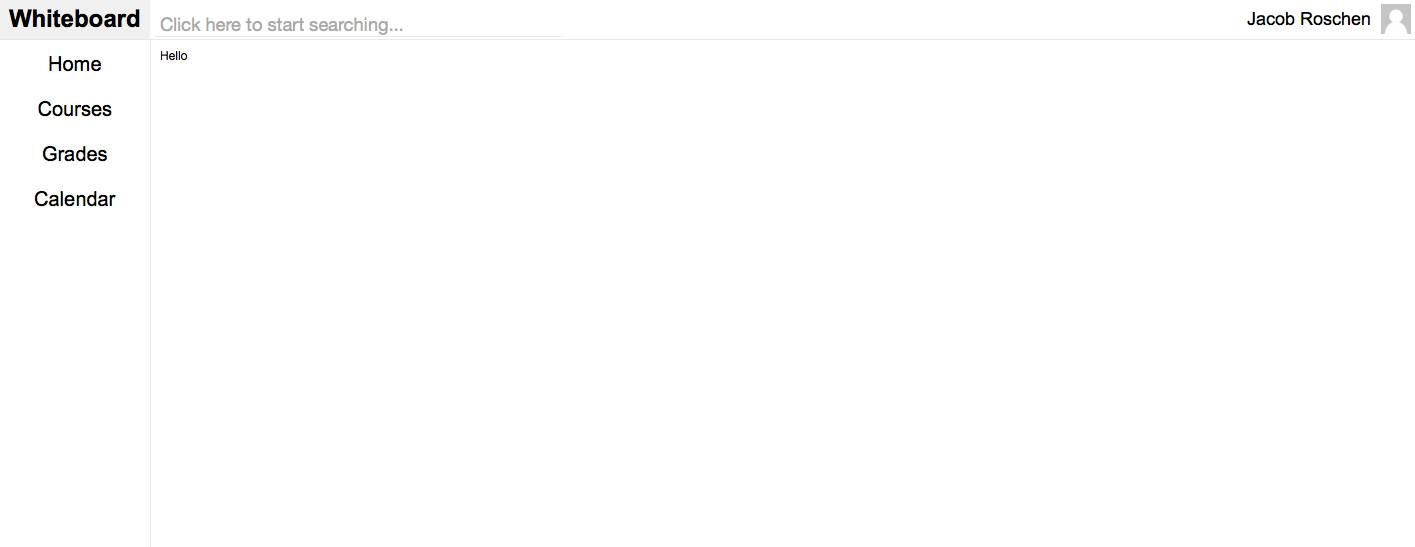
\includegraphics[width=\linewidth]{general_layout}
    \caption{The general layout of the website. This shows the current homepage
    of a user that is logged in.}
    \label{fig:gl}
\end{figure}

\subsection{Login System}

With the open-source library we're using, the PHP-Login project, the
login system is complete. Users can register, and we've set up an email
verification system. Users can log in and the system will remember them.

\subsection{Courses}

Users can search for courses via the search bar, and then they can add and drop
courses. The system keeps track of which users are enrolled in which sections.

\section{Future Plans}

\subsection{Courses UI}

The courses UI could use a little more work for pretty it up and make it
completely intuitive. There is not much more to do in this area, though; much
of the courses UI has already been done.

\subsection{Grades}

\subsection{Announcements and Communication}

The primary aim of announcements and communication is for students to be able
to contact other students in their classes. For simplicity, this will direct to
email. It also will allow teachers to get a list of their students for whole-class
announcements, and for students to get their teachers' emails easily.

\subsection{Professors' UI}

We plan to create a side for professors so that they could do administrative
functions, such as adding students to classes.

\bibliography{refs}{} \bibliographystyle{plain}

\end{document}
